%!TEX root = ../PhDThesis.tex



% *********************************************************************************************************************
\chapter{Introduction}\label{ch:intro}
% *********************************************************************************************************************



\begin{revisedsubmission}[JR-2a: Paragraphs added and existing paragraphs modified to shift focus of the introduction]
As new technologies are introduced and increase in ubiquity they run the chance of being criticised for their impact on social order, and indeed few technologies can escape such a critique of their impact on society.
Devices such as smartphones and smartspeakers are no exception, with examples ranging from popular press (e.g. \citet{Turkle2011}) through to academia (e.g. \citet{Su2015}) identifying troubles with the very act of `using' of devices in the presence of others, identifying myriad negative aspects to such interactions.
These devices are, however, designed such that they \textit{can} be used with ease as part of everyday life, and are pitched as allowing users complete interactions in seconds~\citep{Brown2014}.
%As everyday technology continues to become evermore portable and pervasive, there is a trend to view the encroachment on existing everyday practices with excitement and scepticism.
It is this notion of the problematisation of device use in society, and an academic desire to understand how users \textit{practically} get the devices to work in and through conversation, that motivates the work within this PhD thesis.

% JOEL:: in line with recent discussions, consider reframing this thesis as examining device as a resource in casual social interactions. To acknowledge that it’s not the “work of using the device” that members are concerned with, but more broadly, work of casual social interactions, which just so happens to draw on mobile device use, but just how this mobile device use is done within casual social interaction is the core question. 

This thesis will critically examine casual-social interactions amongst groups of people, and how people engaged in everyday talk draw upon three such technologies: smartphones, smartphones with voice-based personal assistants, and smartspeakers with voice-based personal assistants, as resources within the conversation.
Precisely, the empirical chapters of this thesis unpack the gloss of \textit{what it is to use a device} and \textit{how this is done} while people are collocated with others\footnote{Within related literature the terms \textit{co-located} and \textit{collocated} are often treated as synonymous and interchangeable.
Here, and throughout the thesis, the term \textit{collocated} was arbitrarily used for consistency with publications on which this thesis is based.} in a casual-social setting.

This thesis studies the social interaction around the use of devices in casual-social multiactivity settings, where multiactivity broadly refers to ``the social, interactional and temporal features of situations and conduct in which people organise multiple activities together, concurrently or serially''~\citep[p. 5]{Haddington2014} and in which the members of the setting are involved in multiple activities~\citep{Goffman1968}.
\label{line:casualsocial}This thesis is not the first piece of literature to use the term casual-social setting, with it applied to places for smokers~\citep{Schane2009}, hotel suites~\citep{Pigram1996}, college classrooms~\citep[pp. 30--31]{Yamada1981}, and as places where designers should design mobile interactions for~\citep{Reis2012}.
\citet{St.Lawrence1983} define such a setting as a place where ``people can openly meet and interact with one another''~\citep[p. 42]{St.Lawrence1983}.
Additionally, the definition used in this thesis is also similar although not completely congruent to the notion of ``third places''~\citep{Oldenburg1989}.
Third places are spaces that are outside the home or workplace where people can gather, socialise, and relax.
Casual-social settings expand this definition to include any space, public or private, that is in or outside the home where socialising in a relaxed manner is a primary activity (i.e. the setting has an innate lack of formality one might expect from a work environment).
In the context of this thesis, settings were selected for the fieldwork where the device use would not be considered `out of place', i.e. the device use would be perspicuous to the setting~\citep[p. 181]{Garfinkel2002} and would be expected to unfold.
\end{revisedsubmission}

%\resubmission{Replace broad Ubicomp utopian computing vision introduction with a more focused introduction} %JR-2, PL-DC-A
% In his seminal work, Mark Weiser tendered his vision for the future of ubiquitous computing in which ``the most profound technologies \ldots disappear'' and ``weave themselves into everyday life until they are indistinguishable from it''~\citep{Weiser1991}.
% While mobile technologies, such as smartphones, have indeed become pervasive and impactful in everyday life, they are, as yet, not considered indistinguishable from it by many.
% The use of technology as an embedded activity, specifically when we are collocated with others, has been identified in popular press and academic literature as to problematic~\citep{Su2015}, as distracting~\citep{Lee2016} and replete with distractions~\citep{Nagata2003a}, as isolating us from each other~\citep{Turkle2011}, as leading to a ``mobile bubble''~\citep{Lundgren2013}, and as negatively impacting how we perceive conversation quality~\citep{VandenAbeele2016}.
% Therefore, although the use of electronic devices may indeed be weaved in and through our life, their use remains a prominent source of intrigue and critique.% --- interacting with a device may still be considered remarkable to the lay ethnographer as a distinct activity, and one in which much criticism has been charged.

%This thesis, on the other hand, will critically explore the use of technology \textit{in vivo}, and instead conversely show that using a device in a social setting with others, although problematic at times, can in fact be accomplished with relative ease and will investigate just how people practically accomplish this.
This thesis will critically explore conversations and how the use of technology is interleaved with them \textit{in vivo}, and show that using a device in a social setting with others, although problematic at times, is routinely accomplished in and through everyday conversation.
In order to do this, this thesis adopts an analytic perspective in line with ethnomethodology as defined through the work of \citet{Garfinkel1967}, as well as others within \acf{HCI} and \acf{CSCW} such as \citet{Heath2010,Crabtree2012}.
Adopting this perspective will allow this thesis to show that people can successfully occasion technology use in and through conversation, can \iresubmission{interleave interactions with the device while interacting with others around them}, and can account for and co-manage device interaction collaboratively with co-present others (see \autoref{ch:empirical pub}).
While such a perspective precludes a stance on the \textit{morality} of using devices (see \autoref{ch:background approach}), it does allow for an analytic orientation that reveals that, although the use of devices does engender problematic interactional sequences, these problems are quickly and methodically attended to in and through interaction collaboratively.

Research in related domains such as Mobile \ac{HCI} and \ac{CSCW} has long explored how to design better interactive collocated experiences based around cooperative technology use (e.g. \citet{Lundgren2015}).
Work has explored many different facets of technology use such as augmenting social settings with large screens~\citep{Lucero2012}, making use of mobile applications for souvenir generation~\citep{Durrant2011}, cultural visiting~\citep{Fosh2013}, crowdsourcing video of spectator events~\citep{Flintham2015}, and connecting public displays to benefit public life and communities~\citep{Memarovic2016}.
The work in this thesis, however, is crucially concerned with existing practices of using technology in everyday social interactions; that is, this thesis does not intend to introduce new or augment existing technologies but will study how technology that is already `in-the-wild' is used.
In particular, this concern is with three types of device interaction: touchscreen-based portable device use, \ac{VUI} use with touchscreen-based portable devices, and  \ac{VUI} use with non-port\-able smartspeakers.
Therefore this work, although embedded in the \ac{HCI} domain, pivots more towards studies of work as found in \ac{CSCW}, with a preference for \textit{informing design} through the examination of how people who own or have these devices in their lives make use of them in and through interaction.

The remainder of this chapter will introduce the specific problem-space under examination in this thesis and will identify how the following chapters will attempt to answer the research questions posed.



% *********************************************************************************************************************



\section{Problem definition and space}\label{sec:intro probdef}
It is an increasingly commonplace practice for people to use a device while around others~\citep{Brown2014}, and this is often characterised as leading to problematic or undesirable situations.
Conversely, however, there has been a multitude of positive reasons for technology use identified, such as dealing with anxiety~\citep{Wei2006}, remaining in touch with family members and friends~\citep{Harmon2013}, and information retrieval that is of benefit to the user~\citep{Sohn2008}.
Furthermore, design work has successfully attempted to capitalise on the availability of technology to create collaborative and creative experiences in workplaces, homes, and in public spaces (e.g.~\citet{Fatahgen.Schieck2014c}).
There remains a problem such that, although device use is often characterised as negative, there also is a wide range of positive aspects attributed to it.

Additionally, in spite of considerable progress in mobile technology, critical voices (e.g. \citet{Su2015, Turkle2011}) have pointed out the ways in which the use of devices may isolate people from one another in social situations\iresubmission{, or change the perception of the setting itself.}
On the other hand, socio-technical studies have shown people are skilled at interleaving and \textit{embedding} mobile device use and social interaction in, for example, a living room~\citep{Rooksby2015}, or, in the completion of specific tasks such as collaborative photo-taking setting~\citep{Durrant2011} or mobile search~\citep{Brown2015}.

%\subsection{Studying Settings Naturalistically}\label{sec:intro probdef naturalistic}
The work in this thesis follows on in the traditions of ethnomethodology~\citep{Garfinkel1967}, and indeed adopts ``ethnomethodological indifference''~\citep{Garfinkel1970}, as discussed in \autoref{ch:background approach}.
In introductory terms, this work is not occupied in understanding models of interaction based on theoretical reasoning and considers interaction not only the site of study but the commodity with which the findings are established.
\begin{revisedsubmission}
This precipitates a stance to disregard the adoption of \textit{a priori} theories of interaction in context, instead engendering an approach that involves \textit{going and seeing} what is done to construct meaningful findings from the explication of how individuals use a device as a resource in casual-social interactions.
\end{revisedsubmission}

% JOEL:: in line with recent discussions, consider reframing this thesis as examining device as a resource in casual social interactions. To acknowledge that it’s not the “work of using the device” that members are concerned with, but more broadly, work of casual social interactions, which just so happens to draw on mobile device use, but just how this mobile device use is done within casual social interaction is the core question. 

%\resubmission{Remove references to attention and design implications} %JR-1, PL,1, PL-DC-C, JR-5
%That being said, there are multiple theories surrounding conversation and multiple ongoing activities that come into play when studying interaction.
%Although this thesis will not use such theories in its analyses, it will make these findings available for inspection by researchers in these disciplines through the discussion of transferring the findings into implications for future design work (see \ref{sec:synopsis discussion design}).
%Studies of interaction with artefacts are widespread in disciplines with theoretical perspectives, such as cognitive ergonomics (see \ref{sec:background emca discourse cog}).
%Here, theories such as \ac{DCog} are used to apply an understanding of how cognition is achieved through the sociality of a setting, drawing upon both the present members and its artefacts.
%There are multiple studies which have drawn on \ac{DCog}, with many taking place in safety-critical settings such as clinical and healthcare environments (e.g. \citet{Galliers2007,Blandford2006,Rajkomar2011}) and non-safety critical settings such as the classroom (e.g. \citet{Brown1993}) and interface design research (e.g. \citet{Hollan2000}).
%The adoption of \ac{DCog} as a framework for use in such generative roles is now widespread and shares cross-disciplinary links with efforts to build contextually aware technology (see \ref{sec:background technology mobilehci context}).
%This work does not orient to matters of cognition in this analysis, as the focus is on establishing the accountable actions of members in the setting with no specific task (i.e. this work studies the natural work of an `undirected' interaction where there is no goal being worked towards).
%Yet, however, such theories remain pertinent for consideration.

%Intrinsically, adopting an approach of studying the cognition of members also engenders a reflection upon \textit{cognition} itself, and that of \ac{MWL} and \textit{attention}.
%Complementary research from cognitive ergonomics has extensively studied human attention, types and modality of task, and the demands upon \textit{mental resources} as a result of the task design all as factors relating to predicting \ac{MWL}\footnote{This work is further expanded, with more adequate definitions, later in \autoref{ch:background ehf}.}.
%Much of this work attends to multitasking situations, where humans are dividing their focus between two or more tasks as contiguous work, although recent work, including the lens of \ac{DCog}, facilitates a consideration of the social interaction that occurs in and through task completion.
%The Multiple Resources model~\citep{Wickens2008} denotes ways in which tasks could be designed to allow a person to
%\textit{more successfully}\footnote{The term ``more successfully'' here refers to lower mental workload/demand arising from the performance of the tasks at hand, thus allowing the tasks to be achieved satisfactorily.} accomplish two or more activities simultaneously when the tasks lead to dichotomous mental resources being used, as opposed to shared. For example, a spatial activity uses different resources than a linguistic-related activity, and so a person could more suitably perform the tasks in parallel.
%Conversely, tasks which draw upon conflicting resources, such as two tasks using the auditory modality are less likely to be successful when completed in a dual-task situation.

%With respect to this thesis, in terms of situations where an individual is using their phone with a touch screen and talking with co-present others, it could be speculated that they could more successfully complete this interaction if the tasks being performed draw upon different resources~\citep{Wickens1983}.
%However, the site in which this work is being studied (i.e. a conversation in a casual-social setting) allows members to exhibit a vacillatory focus between activities, which means that such demarcation and analysis is treated as a subjective and reflective exercise in this thesis through the discussion of the findings.
%This thesis will orient to the intersection of device use as it is achieved in, through, and around a multi-party conversation, and uncritically so, will show that device use becomes embedded --- in and inextricable from --- a conversation.
%Ultimately, the thesis will reveal the ways in which members of the conversation interleave their use of a device with their ongoing contingent actions, and \textit{do work} to successfully meet social obligations and norms while they use a device.

%Primarily, this thesis will not posit the use of devices in a conversation as a site of dual-task activity and will in fact adopt a theoretically-agnostic approach\footnote{\citet{Crabtree2000} introduces Ethnomethodologically-informed ethnography, the approach adopted in this thesis, as a method of doing research to uncover interactional accomplishments, as they are \textit{actually} done in and through mundane life.}.
%However, in discussing the findings of the empirical studies conducted, this thesis will draw upon the multiple resources model and \ac{MWL} theories to show the realisation through which members embed device use, and ameliorate social problems with ease, as matters of accomplishment irrespective of the device interaction mode.%\footnote{This, of course, stems from the fact that neither \textit{using a device} or \textit{conversation}, are safety-critical or require sustained attention --- members can and routinely do readjust their orientation as needed throughout interaction.}.
With this theory-agnostic approach in mind, this thesis focuses explicitly on \textit{how} \iresubmission{people accountably use devices as resources in conversation}, and collaborate in and through their device use in casual-social settings while collocated with others.
This work is opposed to making moral judgements and will instead select conversation with device use interleaved within it as a site of study, to reveal \iresubmission{\textit{what} is accomplished in and through the device use, and \textit{how} it is done}.
Although the rhetoric of device interactions as negatively impacting upon a collocated interaction has been established, it loses sight of the individual interactional achievements of members in the settings, which is, as yet, unstudied.

Therefore, in summary, the primary objective of this thesis is to explicate \iresubmission{how and what for purpose devices are brought into ongoing everyday conversations in casual-social settings}.
The need to do this is motivated by the current gap in the literature that exists.
There is nascent work that details the use of devices in such settings as an interactional accomplishment although there remains multiple gloss-like accounts of detrimental device use, which on an interactional level diminishes the work done by members in the setting to make device use accountable and embedded within conversation.
\iresubmission[JR-1, IR-2, ER-1: Remove references to attention literature]{Through the presentation of empirical data which unpacks the work of a relaxed multi-party conversation, this thesis will show how people successfully bring device use into the conversation to accomplish a problem at hand.}
%This thesis will then reflect upon the findings and bring them into context of work in other disciplines that study cognition as an everyday accomplishment.



% *********************************************************************************************************************



\crpagebreak\section{Devices under study}\label{sec:intro devices}
Given the problem defined above, and in line with recent developments with technology, this thesis will examine how interaction unfolds with respect to portable electronic devices such as touchscreen-based smartphones using (1) the touchscreen, and (2) with the voice-based interfaces found on the device.
With regard to the second form of interaction, these \acfp{VUI} are interacted with by talking to the device in a ``conversational'' manner, with the device typically responding back in a `conversational' manner on the screen or through simulated speech\footnote{There is a veritable smorgasbord of different terminologies for these interfaces, such as \textit{Conversational User Interface}, \textit{Conversation(al) Agent}, \textit{Intelligent Personal Assistant}, \textit{Virtual Personal Assistants}, and so on\ldots}, with the device also making use of the \acf{GUI} to display details about the computation and response of the user's request.
%The \ac{VUI} use being studied attend to matters of interaction where the device used by members feature touchscreens and \acfp{GUI}, and thus although the form (or \textit{modality}) of interaction differs, both draw upon visual and touch interaction.
%The second form of interaction involves both visual and touch interaction, in addition to voice-based interaction (a second, or third, modality, depending on your perception).

Furthermore, in line with the development of strictly voice-based interfaces (in the form of smartspeakers), this thesis will further unpack the interactional accomplishment of interleaving interaction with a \ac{VUI} smartspeaker in conversation in the home.
This final form under study in this thesis is where the modality of interaction is restricted solely to voice, i.e. situations where the only way to interact with the device is to talk to it, and for the device to respond with the requested action audibly and/or with synthesised talk.
% In summary, to unpack the interactional accomplishment of members in using each form of device interaction to detail how members embed and collaborate with and through interaction with a device, this thesis will individually study three different devices across three empirical studies:\begin{itemize}
% \item \textbf{visual-touch} interaction mode, where a touchscreen is used as the primary input and output mechanism with a device,
% \item \textbf{hybrid} interaction mode\footnote{Insofar this thesis is concerned, \textit{hybrid} is used as a synonym for \textit{visual-touch-speech}, however, this by no means limits or categorises all devices that do not discretely align as bearing a \textit{visual-touch} or \textit{speech} interaction mode as one-and-the-same.}, where the interaction draws upon the use of touchscreen-based devices that also feature interfaces that can be spoken to, and can respond by synthesising speech,
% \item \textbf{speech} interaction mode, where a device is spoken to using natural language as the primary input mechanism, and the device synthesises speech as a response
% \end{itemize} Pictorially, these three interaction modes can be represented as points on a continuum, as shown in \autoref{fig:intro continuum}.
% This continuum is not presented as a complete continuum, but as a representation of devices under study in this thesis.
% Beyond this, other devices not studied here (e.g. smartwatches) may occupy different positions along the spectrum based on their interaction mode.

\begin{revisedsubmission}[VV-2: Discuss how the different devices are at different stages of mass adoption as a way of linking the studies]
Each of these devices is in different stages of mass adoption, but are widely considered ubiquitous technologies.
Tangentially, theories surrounding the adoption of new technology, such as the `Diffusion of innovations', provide an abstract understanding of technological adoption across society, which provides us with a point of reference to make sense of the how technologies are adopted by consumers at a macro-societal level~\citep{Rogers1995}.
This theory demarcates adopters of technology into arbitrary labels of `innovators', `early adopters', `early' and `late majority' and `laggards', with the latter two categories deemed to be groups who have adopted after the `majority of society'.

Smartphones, at the time writing this thesis (i.e. 2017), have existed for some 20 years, initially as industrial research prototypes before mass adoption.
In the year prior to the first study of this thesis, Ofcom, the United Kingdom's communications regulator, remarked that the UK is now a ``smartphone society'', with 66\% of households having at least one smartphone~\citep[p. 6]{Ofcom2015}, which would classify the smartphone adoption as already in a state of mass adoption.
Conversely, at the time of work being undertaken for the second study, one survey identified personal assistants on portable devices as being used by used by 32\% of respondents in the last year~\citep{AskYourTargetMarket2016}, situating it as in the stage of being adopted by the `early majority'.
Even more so, smartspeakers were included in the UK's household measure of consumer inflation~\citep{ONS2019} a year or so after the underlying research in the third empirical chapter was completed, underscoring their rapid growth and pervasiveness despite only been recently released.

While these labels provide little insight in the context of this thesis' aims to understand the interactional accomplishments of bringing the device use into conversation, they proffer an understanding of the broader \textit{context} in which the device use is brought about.
In other words, they establish the backdrop against which these devices are being studied---each technology studied in this thesis is a pervasive technology that is widely used (and continuing to grow in use).
The use of portable devices is so pervasive that their use regularly features in casual-social settings, as highlighted above by the critiques in literature, and that the use of smartspeakers in the home has rapidly grown to the point where it is included in national measures of inflation just a short time after this thesis was produced.
This thesis does not offer to examine interaction that interleaves the use of all devices in all situations as a definitive study, but merely selects three technologies that are pervasive, have been documented as widely owned and used, and seeks to explicate the ways in which the technology is drawn upon in conversation.
\end{revisedsubmission}
%Furthermore, anecdotally, this continuum also reflects the development of the commercially-available technologies under study, with visual-touch devices being the oldest such devices, and the smartspeakers a relatively recent innovation.

% \begin{figure}[H]
%     \vspace{.5cm}
%     \begin{tikzpicture}
%         \draw [line width = .5mm]  (-4.5,0)  -- (4.5,0);

%         \node[inner sep=0pt] at (-4.5,1.5)
%             {\includegraphics[height=2cm]{Graphics/1-Introduction/ContinuumTouch}};
%         \draw [line width = .5mm]  (-4.5,.125) -- (-4.5,-.125);
%         \node at (-4.5, -.8) {\textbf{Visual-Touch}};

%         \node[inner sep=0pt] at (0,1.5)
%             {\includegraphics[height=2cm]{Graphics/1-Introduction/ContinuumHybrid}};
%         \draw [line width = .5mm]  (0,.125) -- (0,-.125);
%         \node at (0, -.8) {\textbf{Hybrid}};

%         \node[inner sep=0pt] at (4.5,2.5)
%             {
\includegraphics[height=4cm]{Graphics/1-Introduction/ContinuumSpeech}};
%         \draw [line width = .5mm] (4.5,.125) -- (4.5,-.125);
%         \node at (4.5, -.8) {\textbf{Speech}};
%     \end{tikzpicture}
%     \caption[Continuum of the variation of primary device interaction modes being studied.]{Pictorial representation of the variation of primary device interaction modes under study in this thesis as a continuum.}\label{fig:intro continuum}
% \end{figure}



% *********************************************************************************************************************



\section{Research questions}\label{sec:intro rqs}
% JOEL:: in line with recent discussions, consider reframing this thesis as examining device as a resource in casual social interactions. To acknowledge that it’s not the “work of using the device” that members are concerned with, but more broadly, work of casual social interactions, which just so happens to draw on mobile device use, but just how this mobile device use is done within casual social interaction is the core question. 

To answer the gap discussed above, \iresubmission{this thesis will identify what is accomplished through the use of devices in conversation in a casual-social setting and crucially, how this device use is done.
The overarching research question that creates the foundation for this thesis' contributions is:}
\PrintRQ{overall}

\begin{revisedsubmission}
\noindent{}This will be achieved by performing an \iresubmission{ethnographic study of conversations amongst groups of friends socialising together, and orienting to instances where devices are used in and through the conversation}.
By adopting an ethnomethodological lens to fieldwork and analysis (see~\autoref{ch:background approach}), this thesis will show the methods through which members within a setting occasion and embed a device interaction within the wider social context.
This question can be segmented into components that will be answered through the delivery of this ethnographic study.

\end{revisedsubmission}
\PrintRQ{A}
\PrintRQ{B}

% \iresubmission*[New third research question]{Furthermore, and underscoring the main thrust of this thesis, this work will seek to unpack the collaborative achievements of individuals and co-present others to sustain and continually renew the embedded state of using the device within, through, and as a result of the social interaction.
% In line with other ethnographic work in \ac{HCI}, this thesis will harness these findings dentifying how to inform design based on the matters of interaction as identified during the ethnographic work.
% Crucially, this thesis will examine how \textit{technical troubles} arise with the use of devices in conversation, and identify how individuals and groups attend to these as matters:}


% And then say that to do this, this thesis will orient to:
% - How device use is used as a collaborative resource in conversation, to address the members’ problems
% - How troubles with the device use are oriented to and dealt with in interaction


% Furthermore, and underscoring the main thrust of this thesis, this work will seek to unpack the collaborative achievements of individuals and co-present others to sustain and continually renew the embedded state of using the device within, through, and as a result of the social interaction:
% \PrintRQ{2}

\begin{revisedsubmission}
\noindent{}Both of these questions are very much `two sides of the same coin', revealing the nature of how and for what purpose people use a device in conversation.
Therefore, the overall goal of this thesis is to develop an understanding of the efforts of individuals as they interact with each other and bring the use of everyday devices into conversation as a resource to address matters as they arise.
Through this orientation to \textit{what} and \textit{how} this device use unfolds, members' technical troubles with devices may be identified in interaction.
Through this analytic stance, this ethnography will, in turn, identify how individuals and groups attend to these as matters in and through the conversation to accountably organise and accomplish the occasioned activity.

%Overall, these research questions will be answered through the delivery of the ethnographic account of members' accomplishments achieved through the use of the device in interaction, a praxeological account of how members accountably use devices in interaction, and the discussion of how members accountably organise this interaction to accomplish the task at hand.
\end{revisedsubmission}

%A final question of this thesis, once the praxeological account of how interaction with a device is embedded within conversation, and how members perform collaborative action with and around the device interaction, will be to reveal the implications for the design of future collocated experiences with portable devices:
% \iresubmission*[New third research question]{In line with other ethnographic work in \ac{HCI}, this thesis will situate its findings in identifying how to inform design based on the matters of interaction as identified during the ethnographic work.
% Crucially, this thesis will examine how \textit{technical troubles} arise with the use of devices in conversation, and identify how individuals and groups attend to these as matters:}
% %A final question of this thesis, once the praxeological account of how interaction with a device is embedded within conversation, and how members perform collaborative action with and around the device interaction, will be to reveal the implications for the design of future collocated experiences with portable devices:
% \PrintRQ{3}



% *********************************************************************************************************************



\section{Research areas}\label{sec:intro areas}
This thesis adopts an interdisciplinary approach, drawing upon literature, grounding, and practice from several different areas, and in turn, makes a number of contributions (see \ref{sec:intro contributions}) to the different fields:

\begin{itemize}
\item \textit{Ethnomethodology} - Ethnomethodology is the perspective adopted for fieldwork and analysis in this thesis. 
Each of the three studies in this thesis adopt an applied approach to ethnomethodological analysis and explicate the sequential situated action of members in the setting.
%These findings of this thesis include rich descriptions of how members accomplish the work of interleaving device use within conversation in a casual-social setting.
\item \textit{\acf{CSCW}} - Ethnographic studies in \ac{CSCW} provide the groundwork and practical foundation to guide the study of device use as an everyday interactional accomplishment.
Work in \ac{CSCW} also uncovers different facets of mobile device use including qualitative and quantitative studies of mobile device use in everyday life\footnote{Although none---as-yet---serve to reveal the interactional accomplishment of using a device in a casual-social setting, as per the objectives of this thesis.}.
\item \textit{Mobile \acf{HCI}} - There is a plethora of interdisciplinary design work in Mobile \ac{HCI} to create collaborative collocated experiences with everyday portable technologies.
% \item \textit{Cognitive Ergonomics} - This work provides a solid foundation for understanding interaction modalities from a differing but complementary perspective --- the findings from this work will be discussed and linked back to as a reflective exercise.
\end{itemize}



% *********************************************************************************************************************



\section{Contributions}\label{sec:intro contributions}
\begin{revisedsubmission}[ER-3a, JR-3a, ER-2b, ER-2c, ER-3c: Revise the contributions of the thesis]
The Venn diagram in \autoref{fig:intro contributions} shows an approximation of the influence of each of the research areas discussed previously in \ref{sec:intro areas}, based on size.
Furthermore, this diagram shows this thesis' three main contributions and how they are positioned in relation to the areas in which they contribute new knowledge:



\begin{enumerate}[label=\Alph*]
    \item Details of the methodical practice and conduct of people in casual-social settings, detailing how they bring devices into an everyday multi-party conversation, and offering an insight into the differences of how device use is used to address the members' problems that arise in such settings.

    \item Experience and development of the methodological approach in this thesis, both in terms of the application of ethnomethodology and of the nature in which \textit{these technologies} were studied \textit{in these settings}.

    \item Insights of how the interactions unfolded with different technologies and how members undertook work to make these interactional projects collaborative.
    Crucially, through studying interaction with and around such devices, this thesis makes the case for further \ac{CSCW} studies of such settings given their nature of being sites for technology use, and for \ac{HCI} to critically examine and ameliorate the challenges members attend to in using these technologies for their interactional projects.
\end{enumerate}
\end{revisedsubmission}

\begin{figure}[H]
    \centering
    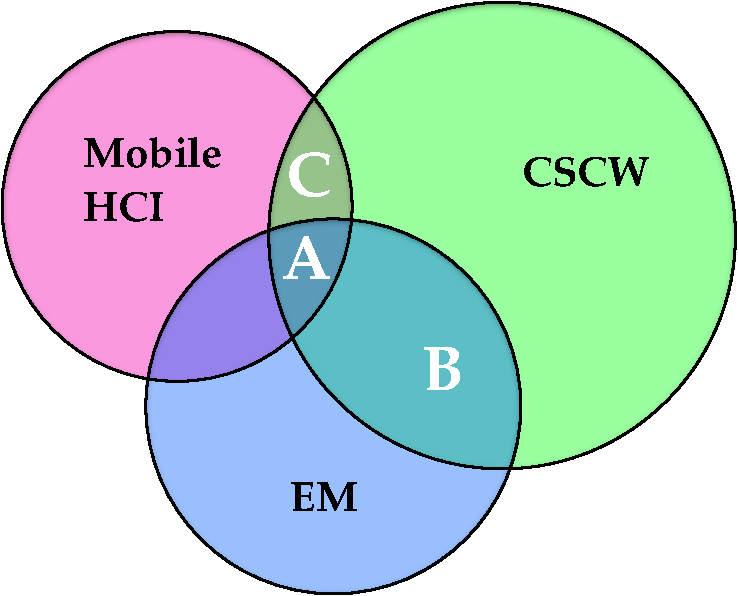
\includegraphics[width=.55\textwidth]{Graphics/1-Introduction/Contributions}
    \caption[Overlap of the different relevant research disciplines and positioning of this thesis' contributions.]{Venn diagram of the influence (size) of the different relevant research areas this thesis draws upon, and how the different multidisciplinary contributions of this work are positioned in relation to each area.}\label{fig:intro contributions}
\end{figure}

% \renewcommand{\theenumi}{\Alph{enumi}}
% \begin{enumerate}

%     \item \textit{Machinery of practices for embedding device interaction in multi-party conversation} --- A praxeological account of the methodical practices employed to embed device interactions in and through contingent social interaction.
%     Furthermore, a rich description of how interacting with devices through visual-touch, voice, and a hybrid-based interface offer and support collaborative efforts amongst members in the setting.
%     This is unpacked and developed through the empirical study and brought together in the discussion (see \ref{sec:synopsis discussion embed}).

%     % \item \textit{Complementing research in existing mental resources literature when exploring non-laboratory use of technology} --- Through the study of interaction with an ethnomethodological analytic lens, this thesis will show how interaction in a non-laboratory setting, such as is the focus of this work, leads to a complex array of interaction modalities being drawn upon and alternated between in quick succession (see \ref{sec:synopsis discussion embed attention}).

%     % \item \textit{Implications for design and study of collocated experiences} --- Based on the study of interaction unfolding with different interaction modes, this thesis will contribute implications for the design and study of collocated interactive experiences, bringing together and juxtaposing the findings from each empirical study (see \ref{sec:synopsis discussion design}).

% \end{enumerate}



% *********************************************************************************************************************



\section{Structure of the thesis}\label{sec:intro structure}
There are \iresubmission{eight} chapters structured over three parts in this thesis, as listed below in \autoref{tab:intro structure}.
A brief summary of each chapter's contribution to the thesis is included in the \textit{Summary} column.

\begin{center}
\vspace{0.5cm}
\begin{longtable}[l]{lp{290pt}}
    \toprule
    \tableheadline{No.}                  & \tableheadline{Summary} \\ \midrule

    \multicolumn{2}{l}{\textbf{\autoref{part:background}: Background and Approach}} \\ \midrule

   \ref{ch:background litreview}     &
   \iresubmission{Continuing the work begun in the Introduction, this chapter lays the groundwork for the thesis by surveying existing literature relating to the use of technology within social and collocated settings, from the perspectives of socio-technical studies, \textit{Mobile \ac{HCI}}, and \textit{\ac{CSCW}}.} \\

   % \ref{ch:background ehf}            &
   %  Relevant literature and theories on interaction modalities, attention, and mental workload from cognitive  perspectives is introduced. \\
    %Although the empirical work undertaken in this thesis does not typically draw on this domain, the findings from this work will be used to contribute new knowledge and practises to \ac{E/HF}, and act as a demonstrator of the contingencies of interaction that an ethnomethodological orientation to analysis reveals.

   \ref{ch:background approach}           &
   \iresubmission{The methodological approach adopted in this thesis is introduced in this chapter.
    Ethnography as a research method is described, and included amongst a brief timeline of the development of ethnomethodological tradition. This provides the context with which the fieldwork and analysis were conducted, and will allow the reader to understand the lens with which this thesis has been produced.} \\ \\
    %The specific practicalities of the approach taken varies based on the particular interaction mode under scrutiny, but the same analytic stance is principally employed in each of the three empirical studies conducted.
    %This chapter will introduce ethnomethodology as a perspective with which the practical and theoretical work in this thesis has adopted, and \ac{EMCA} as an analytic tool used in the orientation to the sequentiality of action of the collected data.
    %This chapter will refrain from practical matters of studying interaction, and focus on the epistemological circumstances of the underlying analysis in this thesis.

    \multicolumn{2}{l}{\textbf{\autoref{part:empirical}: Empirical Work}} \\ \midrule

   \ref{ch:empirical pub}             &
    This chapter presents the study of naturally unfolding interaction with a touchscreen-based portable device within a group of friends socialising together. \\

   \ref{ch:empirical cafe}            &
    This chapter presents a similar study of a group of friends socialising, but where the device interaction is achieved using the \acf{VUI} on the portable device. \\

   \ref{ch:empirical home}            &
    This chapter unpacks how families and friends talk to a \ac{VUI} smartspeaker in the home, with data collected as part of a longitudinal study. \\

    \multicolumn{2}{l}{\textbf{\autoref{part:synopsis}: Synopsis}} \\ \midrule

   \ref{ch:synopsis discussion}       &
    This chapter discusses the findings from the three empirical studies, bringing the findings into the context of existing literature, and how the three independent studies correspondingly reveal the collaborative practices of conversationalists in social settings. \\
    %This chapter will also relate the findings back to the \ac{E/HF} literature uncovered in \autoref{ch:background ehf}, and demonstrate the complexity with which interaction modalities are drawn upon \textit{in vivo}, and the demonstrably need to expand existing knowledge with ethnographic approaches.

   \ref{ch:synopsis conclusions}      &
    This chapter summarises the contributions of this thesis and provides a number of conclusions. \\ \bottomrule

    \caption{Structure of Thesis}\label{tab:intro structure}
\end{longtable}
\end{center}



% *********************************************************************************************************************
